\documentclass[12pt,a4paper]{article}
\usepackage{lmodern}

\usepackage{xcolor}
\usepackage{placeins}
\usepackage{amssymb,amsmath}
\usepackage{ifxetex,ifluatex}
\usepackage{fixltx2e} % provides \textsubscript
\ifnum 0\ifxetex 1\fi\ifluatex 1\fi=0 % if pdftex
  \usepackage[T1]{fontenc}
  \usepackage[utf8]{inputenc}
\else % if luatex or xelatex
  \ifxetex
    \usepackage{mathspec}
    \usepackage{xltxtra,xunicode}
  \else
    \usepackage{fontspec}
  \fi
  \defaultfontfeatures{Mapping=tex-text,Scale=MatchLowercase}
  \newcommand{\euro}{€}
\fi
% use upquote if available, for straight quotes in verbatim environments
\IfFileExists{upquote.sty}{\usepackage{upquote}}{}
% use microtype if available
\IfFileExists{microtype.sty}{%
\usepackage{microtype}
\UseMicrotypeSet[protrusion]{basicmath} % disable protrusion for tt fonts
}{}
\usepackage[lmargin = 2cm, rmargin = 2.5cm, tmargin = 2cm, bmargin =
2.5cm]{geometry}


% Figure Placement:
\usepackage{float}
\let\origfigure\figure
\let\endorigfigure\endfigure
\renewenvironment{figure}[1][2] {
    \expandafter\origfigure\expandafter[H]
} {
    \endorigfigure
}

%%%% Jens %%%%
\usepackage[tiny]{titlesec}
\DeclareMathOperator*{\argmax}{arg\,max}
\DeclareMathOperator*{\argmin}{arg\,min}
\renewcommand{\vec}{\operatorname{vec}}
\newcommand{\tr}{\operatorname{tr}}
\newcommand{\Var}{\operatorname{Var}} % Variance
\newcommand{\VAR}{\operatorname{VAR}} % Vector autoregression
\newcommand{\Lag}{\operatorname{L}} % Lag operator
\newcommand{\Cov}{\operatorname{Cov}}
\newcommand{\diag}{\operatorname{diag}}
\newcommand{\adj}{\operatorname{adj}}
\newcommand{\loglik}{\operatorname{ll}}

\allowdisplaybreaks

\titleformat{\section}
{\normalfont\large\bfseries}{\thesection}{1em}{}

%### sections
\newcommand{\tmpsection}[1]{}
\let\tmpsection=\section
%\renewcommand{\section}[1]{\tmpsection{\underline{#1}} }
\titleformat*{\section}{\large\bfseries}
\titleformat*{\subsection}{\small\bfseries\sffamily}
%\setkomafont{subsection}{\Large}
%\setkomafont{subsubsection}{\large}
%\setkomafont{paragraph}{\large}
%\setkomafont{subparagraph}{\large}





%% citation setup
\usepackage{csquotes}

\usepackage[backend=biber, maxbibnames = 99, style = apa]{biblatex}
\setlength\bibitemsep{1.5\itemsep}
\addbibresource{R_packages.bib}
\usepackage{color}
\usepackage{fancyvrb}
\newcommand{\VerbBar}{|}
\newcommand{\VERB}{\Verb[commandchars=\\\{\}]}
\DefineVerbatimEnvironment{Highlighting}{Verbatim}{commandchars=\\\{\}}
% Add ',fontsize=\small' for more characters per line
\usepackage{framed}
\definecolor{shadecolor}{RGB}{248,248,248}
\newenvironment{Shaded}{\begin{snugshade}}{\end{snugshade}}
\newcommand{\AlertTok}[1]{\textcolor[rgb]{0.94,0.16,0.16}{#1}}
\newcommand{\AnnotationTok}[1]{\textcolor[rgb]{0.56,0.35,0.01}{\textbf{\textit{#1}}}}
\newcommand{\AttributeTok}[1]{\textcolor[rgb]{0.13,0.29,0.53}{#1}}
\newcommand{\BaseNTok}[1]{\textcolor[rgb]{0.00,0.00,0.81}{#1}}
\newcommand{\BuiltInTok}[1]{#1}
\newcommand{\CharTok}[1]{\textcolor[rgb]{0.31,0.60,0.02}{#1}}
\newcommand{\CommentTok}[1]{\textcolor[rgb]{0.56,0.35,0.01}{\textit{#1}}}
\newcommand{\CommentVarTok}[1]{\textcolor[rgb]{0.56,0.35,0.01}{\textbf{\textit{#1}}}}
\newcommand{\ConstantTok}[1]{\textcolor[rgb]{0.56,0.35,0.01}{#1}}
\newcommand{\ControlFlowTok}[1]{\textcolor[rgb]{0.13,0.29,0.53}{\textbf{#1}}}
\newcommand{\DataTypeTok}[1]{\textcolor[rgb]{0.13,0.29,0.53}{#1}}
\newcommand{\DecValTok}[1]{\textcolor[rgb]{0.00,0.00,0.81}{#1}}
\newcommand{\DocumentationTok}[1]{\textcolor[rgb]{0.56,0.35,0.01}{\textbf{\textit{#1}}}}
\newcommand{\ErrorTok}[1]{\textcolor[rgb]{0.64,0.00,0.00}{\textbf{#1}}}
\newcommand{\ExtensionTok}[1]{#1}
\newcommand{\FloatTok}[1]{\textcolor[rgb]{0.00,0.00,0.81}{#1}}
\newcommand{\FunctionTok}[1]{\textcolor[rgb]{0.13,0.29,0.53}{\textbf{#1}}}
\newcommand{\ImportTok}[1]{#1}
\newcommand{\InformationTok}[1]{\textcolor[rgb]{0.56,0.35,0.01}{\textbf{\textit{#1}}}}
\newcommand{\KeywordTok}[1]{\textcolor[rgb]{0.13,0.29,0.53}{\textbf{#1}}}
\newcommand{\NormalTok}[1]{#1}
\newcommand{\OperatorTok}[1]{\textcolor[rgb]{0.81,0.36,0.00}{\textbf{#1}}}
\newcommand{\OtherTok}[1]{\textcolor[rgb]{0.56,0.35,0.01}{#1}}
\newcommand{\PreprocessorTok}[1]{\textcolor[rgb]{0.56,0.35,0.01}{\textit{#1}}}
\newcommand{\RegionMarkerTok}[1]{#1}
\newcommand{\SpecialCharTok}[1]{\textcolor[rgb]{0.81,0.36,0.00}{\textbf{#1}}}
\newcommand{\SpecialStringTok}[1]{\textcolor[rgb]{0.31,0.60,0.02}{#1}}
\newcommand{\StringTok}[1]{\textcolor[rgb]{0.31,0.60,0.02}{#1}}
\newcommand{\VariableTok}[1]{\textcolor[rgb]{0.00,0.00,0.00}{#1}}
\newcommand{\VerbatimStringTok}[1]{\textcolor[rgb]{0.31,0.60,0.02}{#1}}
\newcommand{\WarningTok}[1]{\textcolor[rgb]{0.56,0.35,0.01}{\textbf{\textit{#1}}}}
\usepackage{graphicx}
\makeatletter
\def\maxwidth{\ifdim\Gin@nat@width>\linewidth\linewidth\else\Gin@nat@width\fi}
\def\maxheight{\ifdim\Gin@nat@height>\textheight\textheight\else\Gin@nat@height\fi}
\makeatother
% Scale images if necessary, so that they will not overflow the page
% margins by default, and it is still possible to overwrite the defaults
% using explicit options in \includegraphics[width, height, ...]{}
\setkeys{Gin}{width=\maxwidth,height=\maxheight,keepaspectratio}
\ifxetex
  \usepackage[setpagesize=false, % page size defined by xetex
              unicode=false, % unicode breaks when used with xetex
              xetex]{hyperref}
\else
  \usepackage[unicode=true, linktocpage = TRUE]{hyperref}
\fi
\hypersetup{breaklinks=true,
            bookmarks=true,
            pdfauthor={Jens Klenke},
            pdftitle={R Propädeutikum},
            colorlinks=true,
            citecolor=black,
            urlcolor=black,
            linkcolor=black,
            pdfborder={0 0 0}}
\urlstyle{same}  % don't use monospace font for urls
\setlength{\parindent}{0pt}
\setlength{\parskip}{6pt plus 2pt minus 1pt}
\setlength{\emergencystretch}{3em}  % prevent overfull lines
\setcounter{secnumdepth}{5}

%%% Use protect on footnotes to avoid problems with footnotes in titles
\let\rmarkdownfootnote\footnote%
\def\footnote{\protect\rmarkdownfootnote}

%%% Change title format to be more compact
\usepackage{titling}

% Create subtitle command for use in maketitle
\newcommand{\subtitle}[1]{
  \posttitle{
    \begin{center}\large#1\end{center}
    }
}

\setlength{\droptitle}{-2em}
  \title{R Propädeutikum}
  \pretitle{\vspace{\droptitle}\centering\huge}
  \posttitle{\par}
\subtitle{Lösung Übungsaufgaben 3}
  \author{Jens Klenke}
  \preauthor{\centering\large\emph}
  \postauthor{\par}
  \date{}
  \predate{}\postdate{}

\usepackage{booktabs}
\usepackage{longtable}
\usepackage{array}
\usepackage{multirow}
\usepackage{wrapfig}
\usepackage{float}
\usepackage{colortbl}
\usepackage{pdflscape}
\usepackage{tabu}
\usepackage{threeparttable}
\usepackage{threeparttablex}
\usepackage[normalem]{ulem}
\usepackage{makecell}
\usepackage{xcolor}

%% linespread settings

\usepackage{setspace}

\onehalfspacing


% Language Setup

\usepackage{ifthen}
\usepackage{iflang}
\usepackage[super]{nth}
\usepackage[ngerman, english]{babel}

%Acronyms
\usepackage[printonlyused, withpage, nohyperlinks]{acronym}
\usepackage{changepage}

% Multicols for the Title page
\usepackage{multicol}


% foot


\begin{document}

\selectlanguage{english}

%%%%%%%%%%%%%% Jens %%%%%
\numberwithin{equation}{section}




\restoregeometry


%%% Header 

\begin{minipage}{0.6\textwidth}
Universität Duisburg-Essen\\
Fakultät für Wirtschaftswissenschaften\\
Lehrstuhl für Ökonometrie\\
\end{minipage}

%\begin{minipage}{0.4\textwidth}
	\begin{flushright}
	\vspace{-3cm}
	\includegraphics*[width=5cm]{includes/duelogo_en.png}\\
	\vspace{.125cm}
	\end{flushright}
%\end{minipage}
%\vspace{.125cm}
\hspace{-0.005cm}Wintersemester 2024/2025

\vspace{0.05cm}

\begin{center}
	\vspace{.25cm}
	Jens Klenke \hspace{.5cm}  \\
	\vspace{.25cm}
	\textbf{\Large{R Propädeutikum}}\\
	\vspace{.25cm}
	\textbf{\large{Lösung Übungsaufgaben 3}}\\
	\vspace{.125cm}
\end{center}




% body from markdown

\section{Verteilungen und
Zufallszahlen}\label{verteilungen-und-zufallszahlen}

\subsection{\texorpdfstring{Sei \(X\sim t(5)\). Berechnen Sie
\(P(X<6)\), \(P(3<X\leq7)\) und
\(P(X>4)\).}{Sei X\textbackslash sim t(5). Berechnen Sie P(X\textless6), P(3\textless X\textbackslash leq7) und P(X\textgreater4).}}\label{sei-xsim-t5.-berechnen-sie-px6-p3xleq7-und-px4.}

\begin{itemize}
  \item  $P(X<6)$
\end{itemize}

\begin{Shaded}
\begin{Highlighting}[]
    \FunctionTok{pt}\NormalTok{(}\DecValTok{6}\NormalTok{, }\AttributeTok{df =} \DecValTok{5}\NormalTok{)}
\end{Highlighting}
\end{Shaded}

\begin{verbatim}
## [1] 0.9990769
\end{verbatim}

\begin{itemize}
  \item  $P(3< X \leq 7)$
\end{itemize}

\begin{Shaded}
\begin{Highlighting}[]
    \FunctionTok{pt}\NormalTok{(}\DecValTok{7}\NormalTok{, }\AttributeTok{df =} \DecValTok{5}\NormalTok{) }\SpecialCharTok{{-}} \FunctionTok{pt}\NormalTok{(}\DecValTok{3}\NormalTok{, }\AttributeTok{df =} \DecValTok{5}\NormalTok{)}
\end{Highlighting}
\end{Shaded}

\begin{verbatim}
## [1] 0.01459125
\end{verbatim}

\begin{itemize}
  \item $P(X>4)$.
\end{itemize}

\begin{Shaded}
\begin{Highlighting}[]
    \DecValTok{1} \SpecialCharTok{{-}} \FunctionTok{pt}\NormalTok{(}\DecValTok{4}\NormalTok{, }\AttributeTok{df =} \DecValTok{5}\NormalTok{)}
\end{Highlighting}
\end{Shaded}

\begin{verbatim}
## [1] 0.005161708
\end{verbatim}

\subsection{\texorpdfstring{Berechnen Sie das \(0.95\)-Quantil einer
\(F(4, 5)\)-verteilten
Zufallsvariable.}{Berechnen Sie das 0.95-Quantil einer F(4, 5)-verteilten Zufallsvariable.}}\label{berechnen-sie-das-0.95-quantil-einer-f4-5-verteilten-zufallsvariable.}

\begin{Shaded}
\begin{Highlighting}[]
    \FunctionTok{qf}\NormalTok{(}\FloatTok{0.95}\NormalTok{, }\AttributeTok{df1 =} \DecValTok{4}\NormalTok{, }\AttributeTok{df2 =} \DecValTok{5}\NormalTok{)}
\end{Highlighting}
\end{Shaded}

\begin{verbatim}
## [1] 5.192168
\end{verbatim}

\subsection{Berechnen Sie die Wahrscheinlichkeit dafür, den Jackpot im
Lotto zu gewinnen (d.h. 6 Richtige aus 49). Vernachlässigen Sie bei
Ihrer Berechnung Zusatz- oder Superzahlen. (Hinweis: Benutzen Sie die
hypergeometrische
Verteilung.)}\label{berechnen-sie-die-wahrscheinlichkeit-dafuxfcr-den-jackpot-im-lotto-zu-gewinnen-d.h.-6-richtige-aus-49.-vernachluxe4ssigen-sie-bei-ihrer-berechnung-zusatz--oder-superzahlen.-hinweis-benutzen-sie-die-hypergeometrische-verteilung.}

\begin{Shaded}
\begin{Highlighting}[]
    \FunctionTok{dhyper}\NormalTok{(}\DecValTok{6}\NormalTok{, }\AttributeTok{m =} \DecValTok{6}\NormalTok{, }\AttributeTok{n =} \DecValTok{43}\NormalTok{, }\AttributeTok{k =} \DecValTok{6}\NormalTok{)}
\end{Highlighting}
\end{Shaded}

\begin{verbatim}
## [1] 7.151124e-08
\end{verbatim}

\begin{Shaded}
\begin{Highlighting}[]
    \CommentTok{\# oder per Binomialkoeffizient:}
    \CommentTok{\# 1/choose(49, 6)}
\end{Highlighting}
\end{Shaded}

\subsection{\texorpdfstring{Erzeugen Sie 20 \(\chi^2(5)\)-verteilte
Zufallszahlen ohne (!) dabei die \texttt{rchisq()}-Funktion zu
benutzen.}{Erzeugen Sie 20 \textbackslash chi\^{}2(5)-verteilte Zufallszahlen ohne (!) dabei die rchisq()-Funktion zu benutzen.}}\label{erzeugen-sie-20-chi25-verteilte-zufallszahlen-ohne-dabei-die-rchisq-funktion-zu-benutzen.}

\emph{Hinweis}: \(\chi^2(n)=\sum_{i=1}^n Z_i^2\) mit
\(Z_i\sim\mathcal{N}(0,1)\) für alle \(i=1,...,n\).

\begin{Shaded}
\begin{Highlighting}[]
    \CommentTok{\# seed damit bei beiden Befehlen die Ergebnisse gleich sind}
    \FunctionTok{set.seed}\NormalTok{(}\DecValTok{1549}\NormalTok{) }
    \CommentTok{\# schnell: }
    \FunctionTok{replicate}\NormalTok{(}\DecValTok{20}\NormalTok{, }\FunctionTok{sum}\NormalTok{(}\FunctionTok{rnorm}\NormalTok{(}\DecValTok{5}\NormalTok{)}\SpecialCharTok{\^{}}\DecValTok{2}\NormalTok{))}
\end{Highlighting}
\end{Shaded}

\begin{verbatim}
##  [1]  7.091977  4.967954  5.514013  4.676718  3.931540  7.028298
##  [7] 13.070791  6.461356  7.643946  3.144983  6.943869 10.710932
## [13]  5.536349  6.237411  5.422414  1.965647  3.319014  3.732634
## [19]  8.127858  4.358846
\end{verbatim}

\begin{Shaded}
\begin{Highlighting}[]
    \CommentTok{\# seed damit bei beiden Befehlen die Ergebnisse gleich sind}
    \FunctionTok{set.seed}\NormalTok{(}\DecValTok{1549}\NormalTok{)}
    \CommentTok{\# mit schleife:}
\NormalTok{    rn }\OtherTok{\textless{}{-}} \FunctionTok{numeric}\NormalTok{()}
    \ControlFlowTok{for}\NormalTok{(i }\ControlFlowTok{in} \DecValTok{1}\SpecialCharTok{:}\DecValTok{20}\NormalTok{)\{}
\NormalTok{      rn[i] }\OtherTok{\textless{}{-}} \FunctionTok{sum}\NormalTok{(}\FunctionTok{rnorm}\NormalTok{(}\DecValTok{5}\NormalTok{)}\SpecialCharTok{\^{}}\DecValTok{2}\NormalTok{)}
\NormalTok{    \}}
\NormalTok{    rn}
\end{Highlighting}
\end{Shaded}

\begin{verbatim}
##  [1]  7.091977  4.967954  5.514013  4.676718  3.931540  7.028298
##  [7] 13.070791  6.461356  7.643946  3.144983  6.943869 10.710932
## [13]  5.536349  6.237411  5.422414  1.965647  3.319014  3.732634
## [19]  8.127858  4.358846
\end{verbatim}

\subsection{\texorpdfstring{Ziehen Sie 10-mal standardnormalverteilte
Zufallszahlen vom Umfang \(n = 10000\) und berechnen Sie für jeden
Durchlauf das arithmetische Mittel. Schauen Sie sich danach alle 10
Mittelwerte an. Was fällt Ihnen auf? Sind Sie
überrascht?}{Ziehen Sie 10-mal standardnormalverteilte Zufallszahlen vom Umfang n = 10000 und berechnen Sie für jeden Durchlauf das arithmetische Mittel. Schauen Sie sich danach alle 10 Mittelwerte an. Was fällt Ihnen auf? Sind Sie überrascht?}}\label{ziehen-sie-10-mal-standardnormalverteilte-zufallszahlen-vom-umfang-n-10000-und-berechnen-sie-fuxfcr-jeden-durchlauf-das-arithmetische-mittel.-schauen-sie-sich-danach-alle-10-mittelwerte-an.-was-fuxe4llt-ihnen-auf-sind-sie-uxfcberrascht}

\begin{Shaded}
\begin{Highlighting}[]
\NormalTok{    norm }\OtherTok{\textless{}{-}} \FunctionTok{numeric}\NormalTok{()}
    \ControlFlowTok{for}\NormalTok{(i }\ControlFlowTok{in} \DecValTok{1}\SpecialCharTok{:}\DecValTok{10}\NormalTok{)\{}
\NormalTok{      norm[i] }\OtherTok{\textless{}{-}} \FunctionTok{mean}\NormalTok{(}\FunctionTok{rnorm}\NormalTok{(}\DecValTok{10000}\NormalTok{))}
\NormalTok{    \}}
\NormalTok{    norm}
\end{Highlighting}
\end{Shaded}

\begin{verbatim}
##  [1] -0.007993253  0.000205263 -0.023010730  0.008032737 -0.015314207
##  [6] -0.006583092 -0.010186764 -0.002472349 -0.001919459 -0.006736107
\end{verbatim}

Alle 10 Mittelwerte liegen sehr nahe bei 0. Nicht überraschend, da wir
Zufallszahlen mit Erwartungswert 0 ziehen.

\textbf{Zusatzaufgabe:} Führen Sie dieselbe Simulationsstudie mit
Cauchy-verteilten Zufallszahlen (\texttt{rcauchy()}) durch. Was fällt
Ihnen nun auf? Können Sie sich das Ergebnis erklären?

\begin{Shaded}
\begin{Highlighting}[]
\NormalTok{    cauchy }\OtherTok{\textless{}{-}} \FunctionTok{numeric}\NormalTok{()}
    \ControlFlowTok{for}\NormalTok{(i }\ControlFlowTok{in} \DecValTok{1}\SpecialCharTok{:}\DecValTok{10}\NormalTok{)\{}
\NormalTok{      cauchy[i] }\OtherTok{\textless{}{-}} \FunctionTok{mean}\NormalTok{(}\FunctionTok{rt}\NormalTok{(}\DecValTok{10000}\NormalTok{, }\AttributeTok{df =} \DecValTok{1}\NormalTok{))}
\NormalTok{    \}}
\NormalTok{    cauchy}
\end{Highlighting}
\end{Shaded}

\begin{verbatim}
##  [1]  2.86061674  0.28687124 20.24954554 -2.26699594 -0.93806437
##  [6] -0.09852194  0.06981833  0.03190819  0.16937363  0.36625186
\end{verbatim}

Nun liegen die Mittelwerte nicht wirklich nahe beieinander. Erklärung:
die Cauchy-Verteilung hat keinen Erwartungswert.

\subsection{\texorpdfstring{Zeigen Sie, dass das Integral über die
Dichtefunktion einer \(\chi^2(15)\)-verteilten Zufallsvariable 1
ist.}{Zeigen Sie, dass das Integral über die Dichtefunktion einer \textbackslash chi\^{}2(15)-verteilten Zufallsvariable 1 ist.}}\label{zeigen-sie-dass-das-integral-uxfcber-die-dichtefunktion-einer-chi215-verteilten-zufallsvariable-1-ist.}

\begin{Shaded}
\begin{Highlighting}[]
    \FunctionTok{integrate}\NormalTok{(dchisq, }\AttributeTok{lower =} \DecValTok{0}\NormalTok{, }\AttributeTok{upper =} \ConstantTok{Inf}\NormalTok{, }\AttributeTok{df =} \DecValTok{15}\NormalTok{)}
\end{Highlighting}
\end{Shaded}

\begin{verbatim}
## 1 with absolute error < 1.5e-05
\end{verbatim}

\newpage

\section{Grafiken}\label{grafiken}

\begin{Shaded}
\begin{Highlighting}[]
\FunctionTok{set.seed}\NormalTok{(}\DecValTok{385}\NormalTok{)}
\NormalTok{results }\OtherTok{\textless{}{-}} \FunctionTok{rnorm}\NormalTok{(}\DecValTok{1000}\NormalTok{, }\AttributeTok{mean =} \DecValTok{100}\NormalTok{, }\AttributeTok{sd =} \DecValTok{15}\NormalTok{)}
\end{Highlighting}
\end{Shaded}

\subsection{\texorpdfstring{Kopieren Sie obigen Code und nehmen Sie an,
dass dieser eine IQ-Testreihe mit 1000 Probanden simuliert. Zeichnen Sie
ein Histogramm der Ergebnisse. Geben Sie Ihrem Plot anschließend eine
passende Überschrift sowie passende Achsenbeschriftungen. Spezifizieren
Sie darüber hinaus den Bereich von x- und y-Achse auf \([40,160]\) bzw.
\([0,0.03]\).}{Kopieren Sie obigen Code und nehmen Sie an, dass dieser eine IQ-Testreihe mit 1000 Probanden simuliert. Zeichnen Sie ein Histogramm der Ergebnisse. Geben Sie Ihrem Plot anschließend eine passende Überschrift sowie passende Achsenbeschriftungen. Spezifizieren Sie darüber hinaus den Bereich von x- und y-Achse auf {[}40,160{]} bzw. {[}0,0.03{]}.}}\label{kopieren-sie-obigen-code-und-nehmen-sie-an-dass-dieser-eine-iq-testreihe-mit-1000-probanden-simuliert.-zeichnen-sie-ein-histogramm-der-ergebnisse.-geben-sie-ihrem-plot-anschlieuxdfend-eine-passende-uxfcberschrift-sowie-passende-achsenbeschriftungen.-spezifizieren-sie-daruxfcber-hinaus-den-bereich-von-x--und-y-achse-auf-40160-bzw.-00.03.}

\begin{Shaded}
\begin{Highlighting}[]
    \FunctionTok{set.seed}\NormalTok{(}\DecValTok{385}\NormalTok{)}
\NormalTok{    results }\OtherTok{\textless{}{-}} \FunctionTok{rnorm}\NormalTok{(}\DecValTok{1000}\NormalTok{, }\AttributeTok{mean =} \DecValTok{100}\NormalTok{, }\AttributeTok{sd =} \DecValTok{15}\NormalTok{)}
    \FunctionTok{hist}\NormalTok{(results, }
         \AttributeTok{freq =}\NormalTok{ F,}
         \AttributeTok{xlab =} \StringTok{\textquotesingle{}IQ\textquotesingle{}}\NormalTok{, }
         \AttributeTok{ylab =} \StringTok{\textquotesingle{}Anteil\textquotesingle{}}\NormalTok{, }
         \AttributeTok{main =} \StringTok{\textquotesingle{}Verteilung der IQ{-}Testergebnisse\textquotesingle{}}\NormalTok{, }
         \AttributeTok{xlim =} \FunctionTok{c}\NormalTok{(}\DecValTok{40}\NormalTok{, }\DecValTok{160}\NormalTok{), }
         \AttributeTok{ylim =} \FunctionTok{c}\NormalTok{(}\DecValTok{0}\NormalTok{, }\FloatTok{0.03}\NormalTok{))}
\end{Highlighting}
\end{Shaded}

\begin{center}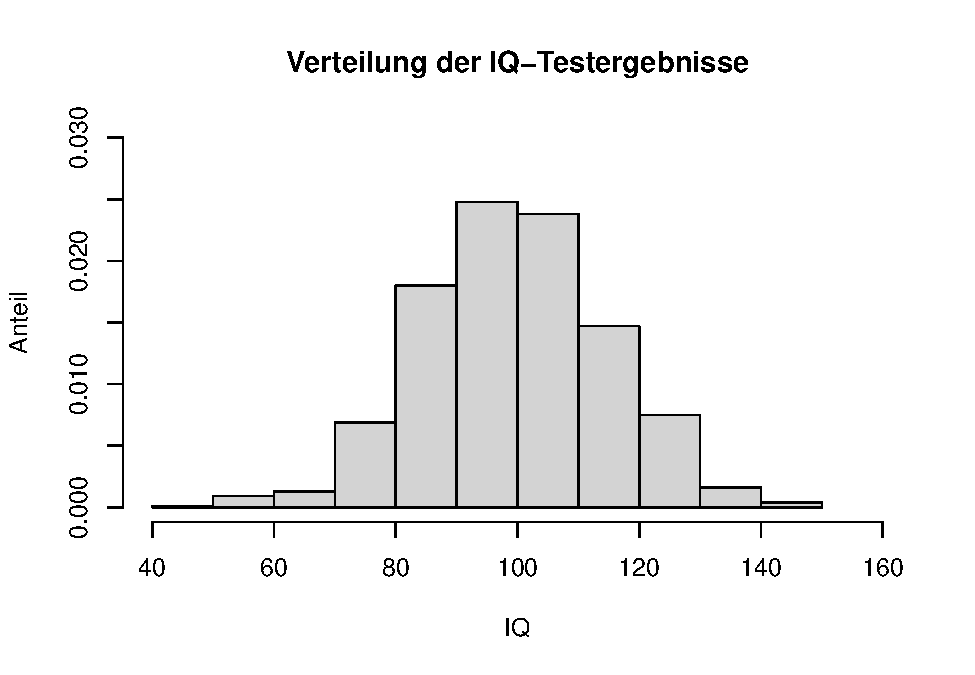
\includegraphics[width=300px]{solution_3_files/figure-latex/unnamed-chunk-12-1} \end{center}

\subsection{\texorpdfstring{Hinterlegen Sie dem Plot die dem IQ
zugrundeliegende, theoretische Dichtefunktion, d.h. eine
Normalverteilung mit \(\mu=100\) und \(\sigma=15\). Wählen Sie als
Zeichenfarbe Rot und machen Sie die einzuzeichnende Linie etwas
breiter.}{Hinterlegen Sie dem Plot die dem IQ zugrundeliegende, theoretische Dichtefunktion, d.h. eine Normalverteilung mit \textbackslash mu=100 und \textbackslash sigma=15. Wählen Sie als Zeichenfarbe Rot und machen Sie die einzuzeichnende Linie etwas breiter.}}\label{hinterlegen-sie-dem-plot-die-dem-iq-zugrundeliegende-theoretische-dichtefunktion-d.h.-eine-normalverteilung-mit-mu100-und-sigma15.-wuxe4hlen-sie-als-zeichenfarbe-rot-und-machen-sie-die-einzuzeichnende-linie-etwas-breiter.}

\begin{Shaded}
\begin{Highlighting}[]
    \FunctionTok{set.seed}\NormalTok{(}\DecValTok{385}\NormalTok{)}
\NormalTok{    results }\OtherTok{\textless{}{-}} \FunctionTok{rnorm}\NormalTok{(}\DecValTok{1000}\NormalTok{, }\AttributeTok{mean =} \DecValTok{100}\NormalTok{, }\AttributeTok{sd =} \DecValTok{15}\NormalTok{)}
    \FunctionTok{hist}\NormalTok{(results, }\AttributeTok{freq =}\NormalTok{ F, }\AttributeTok{xlab =} \StringTok{\textquotesingle{}IQ\textquotesingle{}}\NormalTok{, }\AttributeTok{ylab =} \StringTok{\textquotesingle{}Anteil\textquotesingle{}}\NormalTok{, }
         \AttributeTok{main =} \StringTok{\textquotesingle{}Verteilung der IQ{-}Testergebnisse\textquotesingle{}}\NormalTok{,}
         \AttributeTok{xlim =} \FunctionTok{c}\NormalTok{(}\DecValTok{40}\NormalTok{, }\DecValTok{160}\NormalTok{), }\AttributeTok{ylim =} \FunctionTok{c}\NormalTok{(}\DecValTok{0}\NormalTok{, }\FloatTok{0.03}\NormalTok{))}
\NormalTok{    x }\OtherTok{\textless{}{-}} \FunctionTok{seq}\NormalTok{(}\DecValTok{40}\NormalTok{, }\DecValTok{160}\NormalTok{, }\FloatTok{0.01}\NormalTok{)}
\NormalTok{    y }\OtherTok{\textless{}{-}} \FunctionTok{dnorm}\NormalTok{(x, }\AttributeTok{mean =} \DecValTok{100}\NormalTok{, }\AttributeTok{sd =} \DecValTok{15}\NormalTok{)}
    \FunctionTok{lines}\NormalTok{(x, y, }\AttributeTok{col =} \StringTok{\textquotesingle{}red\textquotesingle{}}\NormalTok{, }\AttributeTok{lwd =} \DecValTok{2}\NormalTok{)}
\end{Highlighting}
\end{Shaded}

\begin{center}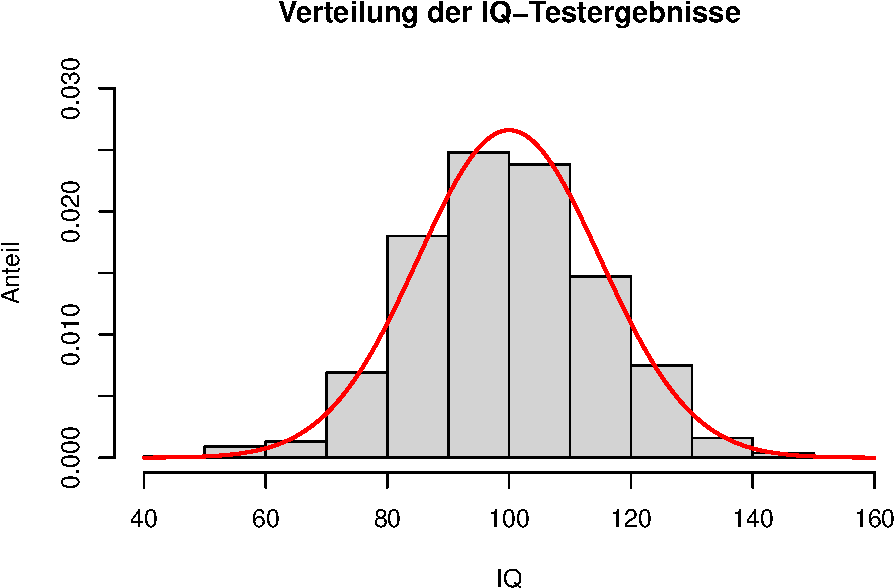
\includegraphics[width=300px]{solution_3_files/figure-latex/unnamed-chunk-13-1} \end{center}

\subsection{Zeichnen Sie einen Punkt in Form eines Dreiecks an das
Maximum der theoretischen Dichte. Wählen Sie als Farbe
Blau.}\label{zeichnen-sie-einen-punkt-in-form-eines-dreiecks-an-das-maximum-der-theoretischen-dichte.-wuxe4hlen-sie-als-farbe-blau.}

\begin{Shaded}
\begin{Highlighting}[]
    \FunctionTok{hist}\NormalTok{(results, }
         \AttributeTok{freq =}\NormalTok{ F, }
         \AttributeTok{xlab =} \StringTok{\textquotesingle{}IQ\textquotesingle{}}\NormalTok{, }
         \AttributeTok{ylab =} \StringTok{\textquotesingle{}Anteil\textquotesingle{}}\NormalTok{, }
         \AttributeTok{main =} \StringTok{\textquotesingle{}Verteilung der IQ{-}Testergebnisse\textquotesingle{}}\NormalTok{, }
         \AttributeTok{xlim =} \FunctionTok{c}\NormalTok{(}\DecValTok{40}\NormalTok{, }\DecValTok{160}\NormalTok{), }
         \AttributeTok{ylim =} \FunctionTok{c}\NormalTok{(}\DecValTok{0}\NormalTok{, }\FloatTok{0.03}\NormalTok{))}
    
\NormalTok{    x }\OtherTok{\textless{}{-}} \FunctionTok{seq}\NormalTok{(}\DecValTok{40}\NormalTok{, }\DecValTok{160}\NormalTok{, }\FloatTok{0.01}\NormalTok{)}
\NormalTok{    y }\OtherTok{\textless{}{-}} \FunctionTok{dnorm}\NormalTok{(x, }\AttributeTok{mean =} \DecValTok{100}\NormalTok{, }\AttributeTok{sd =} \DecValTok{15}\NormalTok{)}
    
    \FunctionTok{lines}\NormalTok{(x, }
\NormalTok{          y, }
          \AttributeTok{col =} \StringTok{\textquotesingle{}red\textquotesingle{}}\NormalTok{, }
          \AttributeTok{lwd =} \DecValTok{2}\NormalTok{)}
    
    \FunctionTok{points}\NormalTok{(}\DecValTok{100}\NormalTok{, }
           \FunctionTok{dnorm}\NormalTok{(}\DecValTok{100}\NormalTok{, }\AttributeTok{mean =} \DecValTok{100}\NormalTok{, }\AttributeTok{sd =} \DecValTok{15}\NormalTok{), }
           \AttributeTok{pch =} \DecValTok{2}\NormalTok{, }
           \AttributeTok{col =} \StringTok{\textquotesingle{}blue\textquotesingle{}}\NormalTok{)}
\end{Highlighting}
\end{Shaded}

\begin{center}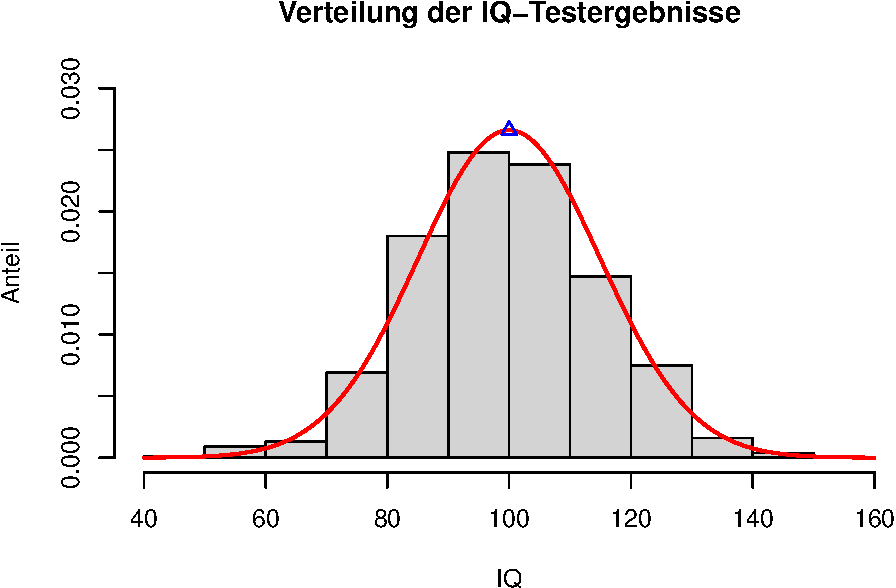
\includegraphics[width=300px]{solution_3_files/figure-latex/unnamed-chunk-14-1} \end{center}

\subsection{\texorpdfstring{Kennzeichnen Sie sowohl das \(0.025\)- als
auch das \(0.975\)-Quantil der theoretischen Dichte, in dem Sie
Vertikalen an diesen Punkten einzeichnen. Wählen Sie als Farbe
Grün.}{Kennzeichnen Sie sowohl das 0.025- als auch das 0.975-Quantil der theoretischen Dichte, in dem Sie Vertikalen an diesen Punkten einzeichnen. Wählen Sie als Farbe Grün.}}\label{kennzeichnen-sie-sowohl-das-0.025--als-auch-das-0.975-quantil-der-theoretischen-dichte-in-dem-sie-vertikalen-an-diesen-punkten-einzeichnen.-wuxe4hlen-sie-als-farbe-gruxfcn.}

\begin{Shaded}
\begin{Highlighting}[]
    \FunctionTok{hist}\NormalTok{(results, }
         \AttributeTok{freq =}\NormalTok{ F, }
         \AttributeTok{xlab =} \StringTok{\textquotesingle{}IQ\textquotesingle{}}\NormalTok{, }
         \AttributeTok{ylab =} \StringTok{\textquotesingle{}Anteil\textquotesingle{}}\NormalTok{, }
         \AttributeTok{main =} \StringTok{\textquotesingle{}Verteilung der IQ{-}Testergebnisse\textquotesingle{}}\NormalTok{, }
         \AttributeTok{xlim =} \FunctionTok{c}\NormalTok{(}\DecValTok{40}\NormalTok{, }\DecValTok{160}\NormalTok{), }
         \AttributeTok{ylim =} \FunctionTok{c}\NormalTok{(}\DecValTok{0}\NormalTok{, }\FloatTok{0.03}\NormalTok{))}
    
\NormalTok{    x }\OtherTok{\textless{}{-}} \FunctionTok{seq}\NormalTok{(}\DecValTok{40}\NormalTok{, }\DecValTok{160}\NormalTok{, }\FloatTok{0.01}\NormalTok{)}
\NormalTok{    y }\OtherTok{\textless{}{-}} \FunctionTok{dnorm}\NormalTok{(x, }\AttributeTok{mean =} \DecValTok{100}\NormalTok{, }\AttributeTok{sd =} \DecValTok{15}\NormalTok{)}
    
    \FunctionTok{lines}\NormalTok{(x, y, }\AttributeTok{col =} \StringTok{\textquotesingle{}red\textquotesingle{}}\NormalTok{, }\AttributeTok{lwd =} \DecValTok{2}\NormalTok{)}
    
    \FunctionTok{points}\NormalTok{(}\DecValTok{100}\NormalTok{, }
           \FunctionTok{dnorm}\NormalTok{(}\DecValTok{100}\NormalTok{, }\AttributeTok{mean =} \DecValTok{100}\NormalTok{, }\AttributeTok{sd =} \DecValTok{15}\NormalTok{), }
           \AttributeTok{pch =} \DecValTok{2}\NormalTok{, }
           \AttributeTok{col =} \StringTok{\textquotesingle{}blue\textquotesingle{}}\NormalTok{)}
    
    \FunctionTok{abline}\NormalTok{(}\AttributeTok{v =} \FunctionTok{qnorm}\NormalTok{(}\FloatTok{0.025}\NormalTok{, }\AttributeTok{mean =} \DecValTok{100}\NormalTok{, }\AttributeTok{sd =} \DecValTok{15}\NormalTok{), }\AttributeTok{col =} \StringTok{\textquotesingle{}green\textquotesingle{}}\NormalTok{)}
    \FunctionTok{abline}\NormalTok{(}\AttributeTok{v =} \FunctionTok{qnorm}\NormalTok{(}\FloatTok{0.975}\NormalTok{, }\AttributeTok{mean =} \DecValTok{100}\NormalTok{, }\AttributeTok{sd =} \DecValTok{15}\NormalTok{), }\AttributeTok{col =} \StringTok{\textquotesingle{}green\textquotesingle{}}\NormalTok{)}
\end{Highlighting}
\end{Shaded}

\begin{center}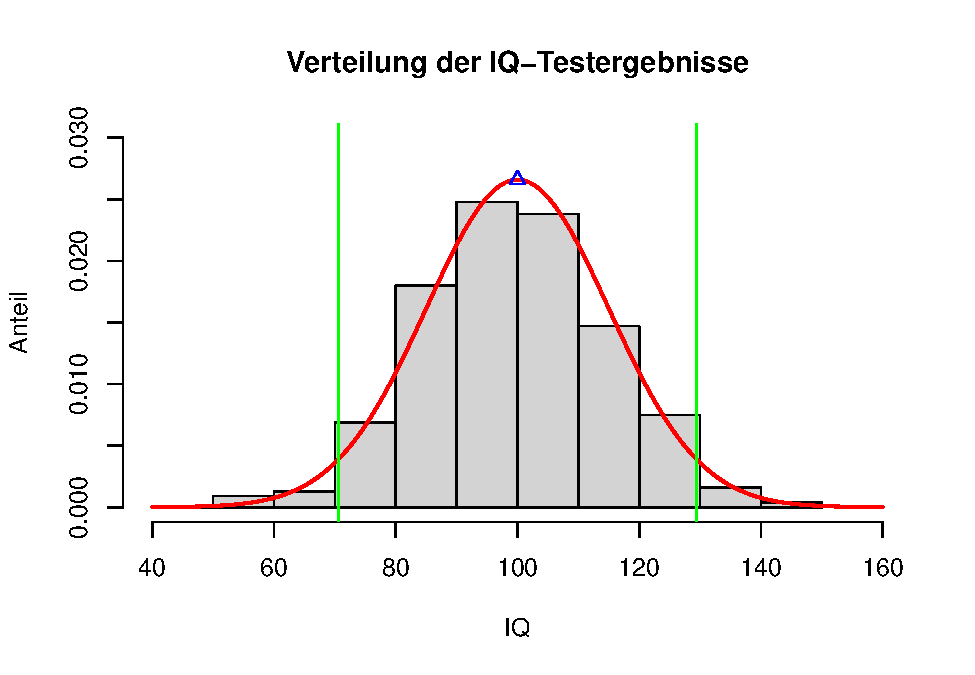
\includegraphics[width=300px]{solution_3_files/figure-latex/unnamed-chunk-15-1} \end{center}

\section{Lineare Regression}\label{lineare-regression}

\subsection{\texorpdfstring{Betrachten Sie im Folgenden den Datensatz
\texttt{faithful}, der Daten zum Old Faithful Geysir im Yellowstone
Nationalpark enthält. Sowohl die Dauer einer Eruption in Min.
(\texttt{eruptions}) als auch die Wartezeit bis zur nächsten Eruption in
Min. (\texttt{waiting}) sind als Variable im Datensatz verfügbar.
Unterstellen Sie nachfolgendes Regressionsmodell und schätzen Sie die
entsprechenden Parameter \(\widehat{\beta_0}\), \(\widehat{\beta_1}\).
Zeichnen Sie anschließend eine geeignete Grafik und interpretieren Sie
diese.}{Betrachten Sie im Folgenden den Datensatz faithful, der Daten zum Old Faithful Geysir im Yellowstone Nationalpark enthält. Sowohl die Dauer einer Eruption in Min. (eruptions) als auch die Wartezeit bis zur nächsten Eruption in Min. (waiting) sind als Variable im Datensatz verfügbar. Unterstellen Sie nachfolgendes Regressionsmodell und schätzen Sie die entsprechenden Parameter \textbackslash widehat\{\textbackslash beta\_0\}, \textbackslash widehat\{\textbackslash beta\_1\}. Zeichnen Sie anschließend eine geeignete Grafik und interpretieren Sie diese.}}\label{betrachten-sie-im-folgenden-den-datensatz-faithful-der-daten-zum-old-faithful-geysir-im-yellowstone-nationalpark-enthuxe4lt.-sowohl-die-dauer-einer-eruption-in-min.-eruptions-als-auch-die-wartezeit-bis-zur-nuxe4chsten-eruption-in-min.-waiting-sind-als-variable-im-datensatz-verfuxfcgbar.-unterstellen-sie-nachfolgendes-regressionsmodell-und-schuxe4tzen-sie-die-entsprechenden-parameter-widehatbeta_0-widehatbeta_1.-zeichnen-sie-anschlieuxdfend-eine-geeignete-grafik-und-interpretieren-sie-diese.}

\begin{align*}
  \text{waiting}_t = \beta_0+\beta_1 \text{eruptions}_t + u_t 
\end{align*}

\begin{Shaded}
\begin{Highlighting}[]
\NormalTok{    model\_ff }\OtherTok{\textless{}{-}} \FunctionTok{lm}\NormalTok{(waiting }\SpecialCharTok{\textasciitilde{}}\NormalTok{ eruptions, }\AttributeTok{data =}\NormalTok{ faithful)}
   
    \FunctionTok{plot}\NormalTok{(faithful}\SpecialCharTok{$}\NormalTok{eruptions, }
\NormalTok{         faithful}\SpecialCharTok{$}\NormalTok{waiting, }
         \AttributeTok{xlab =} \StringTok{\textquotesingle{}Dauer einer Eruption (in Min.)\textquotesingle{}}\NormalTok{,}
         \AttributeTok{ylab =} \StringTok{\textquotesingle{}Wartezeit zur nächsten Eruption (in Min.)\textquotesingle{}}\NormalTok{)}
    
    \FunctionTok{abline}\NormalTok{(model\_ff, }\AttributeTok{col =} \StringTok{\textquotesingle{}red\textquotesingle{}}\NormalTok{)}
\end{Highlighting}
\end{Shaded}

\begin{center}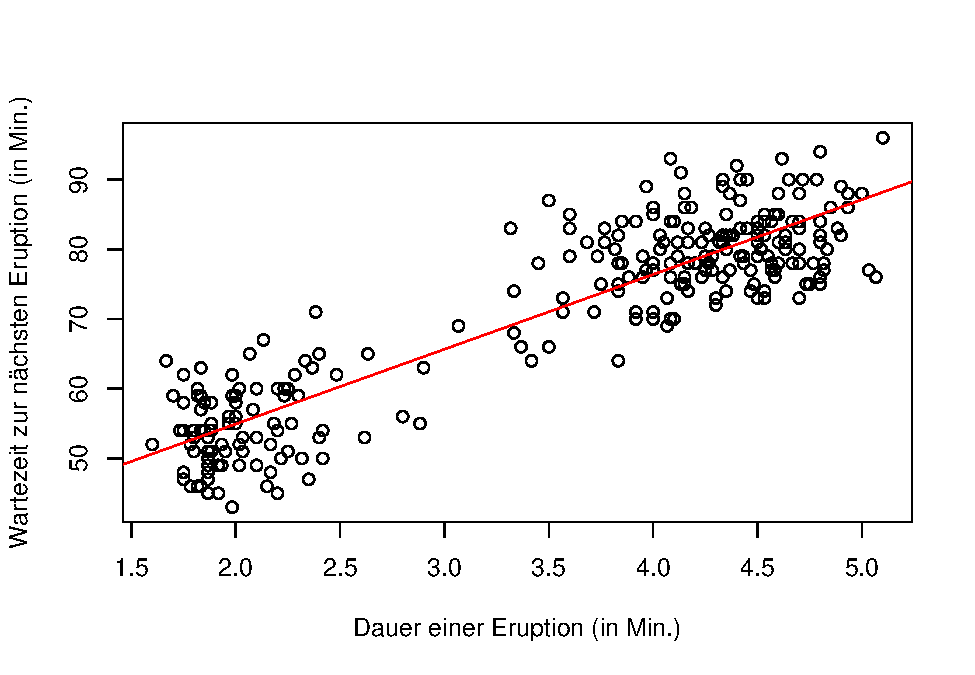
\includegraphics[width=300px]{solution_3_files/figure-latex/unnamed-chunk-16-1} \end{center}

Grundsätzlich: Je länger die Dauer einer Eruption ist, desto länger ist
die Wartezeit bis zur nächsten Eruption.

\subsection{\texorpdfstring{Verschaffen Sie sich mit \texttt{summary()}
einen Überblick über ihr in 3.1 erhaltenes Ergebnis. Interpretieren Sie
die geschätzten Koeffizienten und speichern Sie anschließend das \(R^2\)
(\emph{Multiple R-squared}) in der Variablen \texttt{R2} ab. (Hinweis:
Schauen Sie sich die, beim Ausführen von \texttt{summary()}, ausgegebene
Datenstruktur genauer
an.)}{Verschaffen Sie sich mit summary() einen Überblick über ihr in 3.1 erhaltenes Ergebnis. Interpretieren Sie die geschätzten Koeffizienten und speichern Sie anschließend das R\^{}2 (Multiple R-squared) in der Variablen R2 ab. (Hinweis: Schauen Sie sich die, beim Ausführen von summary(), ausgegebene Datenstruktur genauer an.)}}\label{verschaffen-sie-sich-mit-summary-einen-uxfcberblick-uxfcber-ihr-in-3.1-erhaltenes-ergebnis.-interpretieren-sie-die-geschuxe4tzten-koeffizienten-und-speichern-sie-anschlieuxdfend-das-r2-multiple-r-squared-in-der-variablen-r2-ab.-hinweis-schauen-sie-sich-die-beim-ausfuxfchren-von-summary-ausgegebene-datenstruktur-genauer-an.}

\begin{Shaded}
\begin{Highlighting}[]
    \FunctionTok{summary}\NormalTok{(model\_ff)}
\end{Highlighting}
\end{Shaded}

\begin{verbatim}
## 
## Call:
## lm(formula = waiting ~ eruptions, data = faithful)
## 
## Residuals:
##      Min       1Q   Median       3Q      Max 
## -12.0796  -4.4831   0.2122   3.9246  15.9719 
## 
## Coefficients:
##             Estimate Std. Error t value Pr(>|t|)    
## (Intercept)  33.4744     1.1549   28.98   <2e-16 ***
## eruptions    10.7296     0.3148   34.09   <2e-16 ***
## ---
## Signif. codes:  0 '***' 0.001 '**' 0.01 '*' 0.05 '.' 0.1 ' ' 1
## 
## Residual standard error: 5.914 on 270 degrees of freedom
## Multiple R-squared:  0.8115, Adjusted R-squared:  0.8108 
## F-statistic:  1162 on 1 and 270 DF,  p-value: < 2.2e-16
\end{verbatim}

\begin{itemize}
  \item Achsenabschnitt (\texttt{Intercept})
  \begin{itemize}
    \item Bei einer Eruptionsdauer von 0 Minuten, beträgt die Wartezeit bis zur nächsten Eruption etwa 33.5 Minuten (nicht wirklich sinnvoll interpretierbar).
  \end{itemize}
  \item Steigungskoeffizient (\texttt{eruptions})
  \begin{itemize}
    \item Steigt die Dauer einer Eruption um eine Minute, steigt die Wartezeit bis zur nächsten Eruption um etwa 10.7 Minuten.
  \end{itemize}
\end{itemize}

\begin{Shaded}
\begin{Highlighting}[]
\NormalTok{    R2 }\OtherTok{\textless{}{-}} \FunctionTok{summary}\NormalTok{(model\_ff)}\SpecialCharTok{$}\NormalTok{r.squared}
\NormalTok{    R2}
\end{Highlighting}
\end{Shaded}

\begin{verbatim}
## [1] 0.8114608
\end{verbatim}

Summary erstellt ebenfalls eine Liste, in der u. a. auch das \(R^2\)
enthalten ist.

\subsection{\texorpdfstring{Angenommen Sie beobachten einen zusätzlichen
Datenpunkt für die Dauer einer Eruption von \(X_{new}=4\). Sagen Sie die
entsprechende Wartezeit bis zur nächsten Eruption
vorher.}{Angenommen Sie beobachten einen zusätzlichen Datenpunkt für die Dauer einer Eruption von X\_\{new\}=4. Sagen Sie die entsprechende Wartezeit bis zur nächsten Eruption vorher.}}\label{angenommen-sie-beobachten-einen-zusuxe4tzlichen-datenpunkt-fuxfcr-die-dauer-einer-eruption-von-x_new4.-sagen-sie-die-entsprechende-wartezeit-bis-zur-nuxe4chsten-eruption-vorher.}

\begin{Shaded}
\begin{Highlighting}[]
\NormalTok{    new\_value }\OtherTok{\textless{}{-}} \FunctionTok{data.frame}\NormalTok{(}\AttributeTok{eruptions =} \DecValTok{4}\NormalTok{)}
    \FunctionTok{predict}\NormalTok{(model\_ff, }\AttributeTok{newdata =}\NormalTok{ new\_value)}
\end{Highlighting}
\end{Shaded}

\begin{verbatim}
##        1 
## 76.39296
\end{verbatim}

Bei einer Eruptionsdauer von 4 Min. beträgt die mit unserem Modell
geschätzte Wartezeit etwa. 76.4 Min.

\end{document}
